\documentclass[unicode,11pt,notheorems]{beamer}

\usepackage[T2A]{fontenc}
\usepackage[utf8]{inputenc}
\usepackage[russian]{babel}
\usepackage{amsmath,amsfonts,amssymb,amsthm}
\usepackage{mathtools}

\usepackage{colortbl,tabularx,array}
\usepackage{ulem}
\usepackage{tikz, graphicx}

%\usepackage{tkz-graph}
\usetikzlibrary{positioning,arrows,calc}
\usetikzlibrary{petri}
\usetikzlibrary{decorations.pathreplacing}

%Описание стиля презентации
\usetheme[sidebar=0]{kfmn} 
\setbeamercovered{transparent}

%[0, 6, 8, 8, 10, 5, 6, 10, 8, 10, 10], 

\pgfdeclareimage[height=8mm]{university-logo}{logo-iem.png}
\logo{\pgfuseimage{university-logo}}
%2[0, 11, 10, 8, 11, 5, 11, 11, 8, 11, 10, 11],

\titlepicture{
	\begin{tikzpicture}[y=1.4cm,overlay,rotate=8]
	\coordinate (O) at (-3cm,0.9cm);
	\filldraw[thick,draw= vgublue, fill=vgublue!20!white] (0,0) circle[radius=4.2cm];
	\clip (0,0) circle[radius=4.2cm];
	\draw (-1.5,1.5) node{
	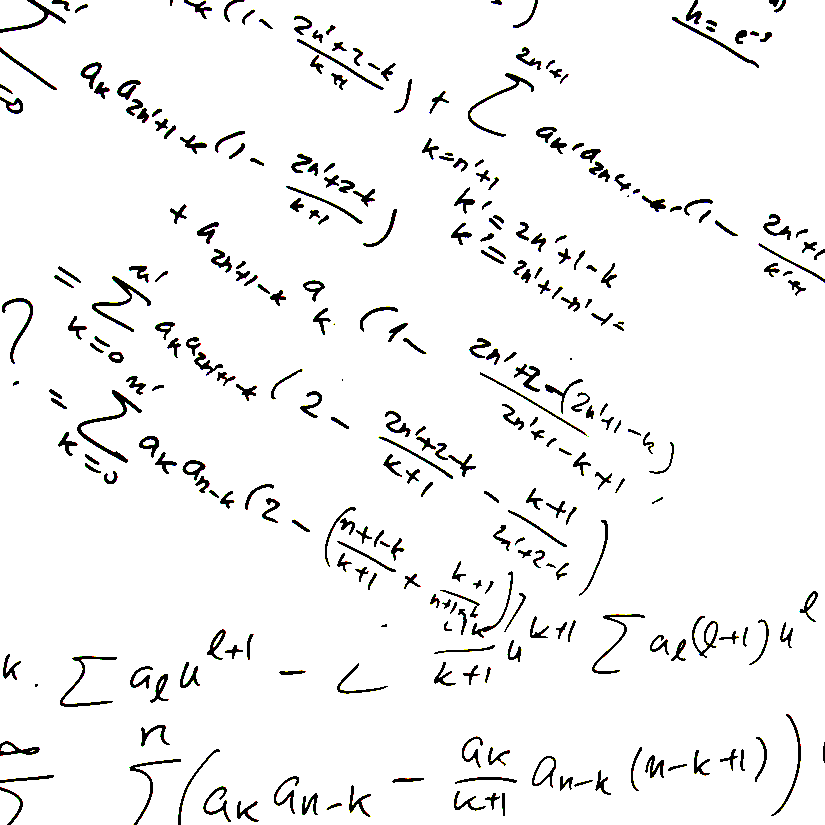
\includegraphics[width=8cm]{titlepic.png}
	};
\end{tikzpicture}
}

\usepackage[math]{iwona}

\newcommand{\hplus}{\mathbin{\hat+}}
\newcommand{\hdot}{\mathbin{\hat\cdot}}
% Описание теорем
\newtheorem{theorem}{Теорема}
\newtheorem{seq}{Следствие}
%%

%\VKR
\LECT % можно ещё лекцию забацать.
%\REPORT % можно ещё лекцию забацать.

%\titlepicture{
%%	\begin{tikzpicture}[overlay]
%%			\draw[opacity=0.4]  (-0.3,1.8) node {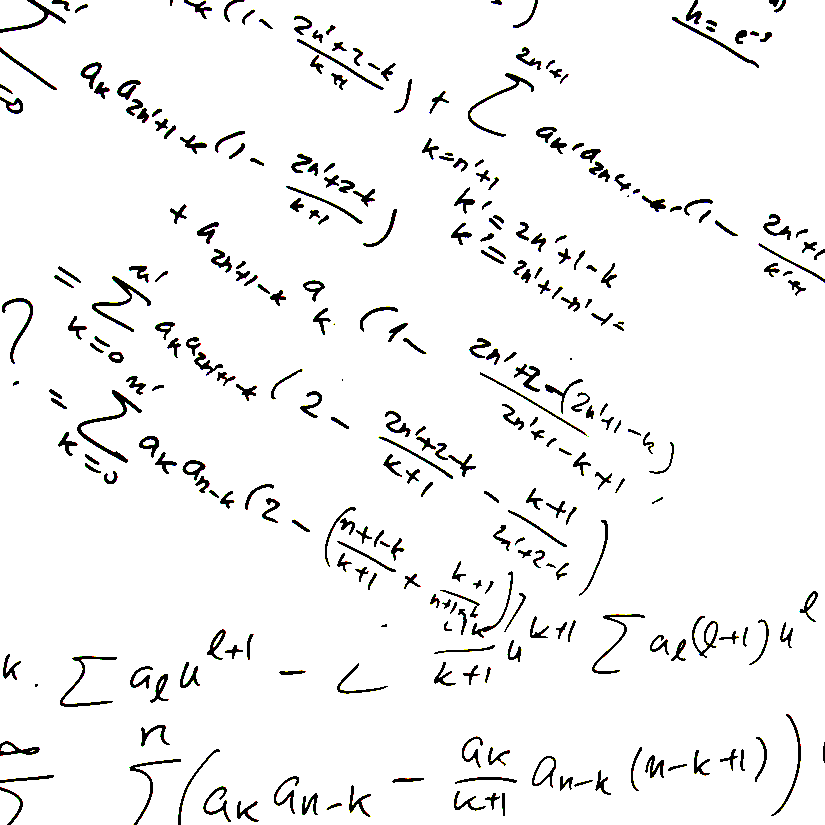
\includegraphics[width=3.5cm]{titlepic.png}};
%%	\end{tikzpicture}
%}

% Титульный лист теорем
\author[Д.\,В. Чупраков]{канд.\,физ.-матем.\,наук, доцент Д.\,В. Чупраков\\[6pt] usr10381@vyatsu.ru}

\institute[ВятГУ]{ФГБОУ ВО Вятский государственный университет}

\department{Факультет экономики и финансов}

\title[Графы и сети]{
	Введение в экономико-математическое моделирование\\[12pt]
	Лекция 2. Графы и сети}
\subtitle{Анализ и оптимизация сетевой модели}


\date{16 апреля 2020 г.}


%\setbeamercolor{coloredboxstuff}{fg=yellow,bg=white!10!blue}

\setbeamercovered{invisible}


\tikzset{
	 myarrow/.style={->, >=latex', shorten >=1pt, thick}
}



\tikzset{add/.style n args={4}{
    minimum width=6mm,
    path picture={
        \draw[black] 
            (path picture bounding box.south east) -- (path picture bounding box.north west)
            (path picture bounding box.south west) -- (path picture bounding box.north east);
        \node at ($(path picture bounding box.south)+(0,0.13)$)     {\tiny #1};
        \node at ($(path picture bounding box.west)+(0.13,0)$)      {\tiny #2};
        \node at ($(path picture bounding box.north)+(0,-0.13)$)        {\tiny #3};
        \node at ($(path picture bounding box.east)+(-0.13,0)$)     {\tiny #4};
        }
    }
}

\tikzset{bigadd/.style n args={4}{
    minimum width=20mm,
    path picture={
        \draw[black] 
            (path picture bounding box.south east) -- (path picture bounding box.north west)
            (path picture bounding box.south west) -- (path picture bounding box.north east);
        \node at ($(path picture bounding box.south)+(0,0.5)$)     { #1};
        \node at ($(path picture bounding box.west)+(0.5,0)$)      {#2};
        \node at ($(path picture bounding box.north)+(0,-0.5)$)        {#3};
        \node at ($(path picture bounding box.east)+(-0.5,0)$)     {#4};
        }
    }
}
\begin{document}


\maketitle

\begin{frame}{Структура лекции}
	\tableofcontents
\end{frame}


\section{Исследование сетевой модели}
\subsection{Временные параметры}

\begin{frame}{Временн\'{ы}е параметры событий}
	\begin{itemize}
	\item[$t_\text{р}(i)$]~--- 
		ранний (ожидаемый) срок свершения $i$-го события: 
		$$\alert{t_\text{р}(i) = \max\limits_{j}\big(t_\text{р}(j)+t(j,i)\big)}$$

	\item[$t_\text{п}(i)$]~--- 
		поздний (предельный) срок: 
		$$\alert{t_\text{п}(i) = \min\limits_{j}\big(t_\text{п}(j)-t(i,j)\big)}$$
 	
	\item[$R(i)$]~--- 			
		резерв времени  i-го события:
		$$\alert{R(i)=t_\text{п}(i) - t_\text{р}(i)}$$
	\end{itemize}

	\structure{Изображение события:}\quad
\begin{tikzpicture}[baseline]
	\node[minimum height=2cm,draw,circle,bigadd={$i$}{$t_\text{р}(i)$}{$R(i)$}{$t_\text{п}(i)$}] (P0) at (0,0) {};
\end{tikzpicture}
\end{frame}
%	\medskip
%	\structure{Частные случаи:}
%	\begin{itemize}
%	\item ранний и поздний сроки свершения исходного события~--- 0
%	
%	\item поздний срок свершения завершающего события~--- продолжительность  критического пути.
%
%%	\item[$t_\text{п}(i)$]~--- 
%%		поздний (предельный) срок: 
%%		$t_\text{п}(i) = \min\limits_{i,j}(t_\text{п}(j)-t(i,j))$.
%% 	
%%	\item[$R(i)$]~--- 			
%%		резерв времени  i-го события:
%%		$R(i)=t_\text{п}(i) - t_\text{р}(i)$
%	\end{itemize}



\begin{frame}{Временн\'{ы}е параметры работ}

\begin{tikzpicture}[>=latex]

	\draw [->,thick] (0,0) -- (11,0) node[below]{$t$};
	\draw [very thick,vgublue] 
			(1,1) 
			+(0,0.2) -- +(0,-0.2) 
			+(0,0) -- ++(2,0) node [midway,text width=1.9cm,align=center,below] {\footnotesize Момент события $i$\par}
			+(0,0.2) -- +(0,-0.2);
	\draw [very thick,vgublue] 
			(8,2) 
			+(0,0.2) -- +(0,-0.2) 
			+(0,0) -- ++(2,0)  node [midway,text width=1.9cm,align=center,below] {\footnotesize Момент события $j$\par}
			+(0,0.2) -- +(0,-0.2);

	\draw [dashed] 
			(1,1) 
			+(0,0)-- +(0,-1) node[below,vgublue]{$t_\text{р}(i)$}
			++(2,0) -- +(0,-1) node[below,vgublue]{$t_\text{п}(i)$}
			(8,2) 
			+(0,0)-- +(0,-2) node[below,vgublue]{$t_\text{р}(j)$}
			++(2,0) -- +(0,-2) node[below,vgublue]{$t_\text{п}(j)$}
			;

	\draw [thick,vgured, >->] 
			(1,1.05) 
			+(0,0) -- +(5,0) 
			;
	\draw [decorate,decoration={brace,amplitude=10pt},xshift=0pt,yshift=1mm]
			(1,1) 
			+(0,0) -- +(5,0)   node [black,midway,yshift=0.6cm,vgured] {$t(i,j)$}
			;
			
	\draw [thick,vgured, >->] 
			(8,2.05) 
			+(-3,0) -- +(2,0) 
			;
	\draw [decorate,decoration={brace,amplitude=10pt},xshift=0pt,yshift=1mm]
			(8,2) 
			+(-3,0) -- +(2,0)   node [black,midway,yshift=0.6cm,vgured] {$t(i,j)$}
			;
	\draw [dashed] 
			(1,1) 
			+(0,0)-- +(0,-1) node[below,vgublue]{$t_\text{р}(i)$}
			++(2,0) -- +(0,-1) node[below,vgublue]{$t_\text{п}(i)$}
			(8,2) 
			+(0,0)-- +(0,-2) node[below,vgublue]{$t_\text{р}(j)$}
			++(2,0) -- +(0,-2) node[below,vgublue]{$t_\text{п}(j)$}
			;

	\draw [dashed] 
			(1,1) 
			+(0,0)-- +(0,-1) node[below,vgured,yshift=-4mm]{$t_\text{рн}(i,j)$}
			+(5,0)-- +(5,-1) node[below,vgured,yshift=-4mm]{$t_\text{ро}(i,j)$}
			(8,2) 
			+(2,0)-- +(2,-2) node[below,vgured,yshift=-4mm]{$t_\text{по}(i,j)$}
			+(-3,0)-- +(-3,-2) node[below,vgured]{$t_\text{пн}(i,j)$}
			;
	\end{tikzpicture}	

\bigskip
	\begin{itemize}
	\item[$t_\text{рн}(i,j)$]~--- 
		ранний срок начала работы: \hfill
		$\alert{t_\text{рн}(i,j)=t_\text{р}(i)}$

	\item[$t_\text{ро}(i,j)$]~--- 
		ранний срок окончания работы:  \hfill
		$\alert{t_\text{ро}(i,j)=t_\text{р}(i)+t(i,j)}$

	\item[$t_\text{пн}(i,j)$]~--- 
		поздний срок начала работы:  \hfill
		$\alert{t_\text{пн}(i,j)=t_\text{п}(i)-t(i,j)}$

	\item[$t_\text{по}(i,j)$]~--- 
		поздний срок окончания работы:  \hfill
		$\alert{t_\text{по}(i,j)=t_\text{п}(j)}$
	\end{itemize}
\end{frame}

\begin{frame}{Резервы времени}
\begin{tikzpicture}[>=latex]

	\draw [->,thick] (0.5,0) -- (11.5,0) node[above]{$t$};
	\draw [very thick,vgublue] 
			(1,1) 
			+(0,0.2) -- +(0,-0.2) 
			+(0,0) -- ++(2,0) node [midway,text width=1.9cm,align=center,below] {\footnotesize Момент события $i$\par}
			+(0,0.2) -- +(0,-0.2);
	\draw [very thick,vgublue] 
			(9,3) 
			+(0,0.2) -- +(0,-0.2) 
			+(0,0) -- ++(2,0)  node [midway,text width=1.9cm,align=center,below] {\footnotesize Момент события $j$\par}
			+(0,0.2) -- +(0,-0.2);

	\draw [dashed] 
			(1,3) 
			+(0,0)-- +(0,-3) node[below,vgublue]{$t_\text{р}(i)$}
			++(2,0) -- +(0,-3) node[below,vgublue]{$t_\text{п}(i)$}
			++(3,0) -- +(0,-3)
			++(2,0) -- +(0,-3)
			(9,3) 
			+(0,0)-- +(0,-3) node[below,vgublue]{$t_\text{р}(j)$}
			++(2,0) -- +(0,-3) node[below,vgublue]{$t_\text{п}(j)$}


			;

	\draw [thick,vgugreen, >->] 
			(1,1.1) 
			+(0,0) -- +(5,0) 
			;
			
	\draw [thick,vgugreen, >->] 
			(6,3.1) 
			+(-3,0) -- +(2,0) 
			;

	\draw [vgured,decorate,decoration={brace,amplitude=10pt},xshift=0pt,yshift=1mm]
			(6,1) 
			+(5,0) -- +(0,0)   node [black,midway,yshift=-0.6cm,vgured] 
			{\small $R_\text{п}(i,j)$}
			;
	\draw [vgured,decorate,decoration={brace,amplitude=10pt},xshift=0pt,yshift=1mm]
			(6,1) 
			+(0,0) -- +(3,0)   node [black,midway,yshift=0.6cm,vgured] 
			{\small $R_\text{с}(i,j)$}
			;
	\draw [vgured,decorate,decoration={brace,amplitude=10pt},xshift=0pt,yshift=1mm]
			(8,3) 
			+(0,0) -- +(3,0)   node [black,midway,yshift=0.6cm,vgured] 
			{\small $R_\text{1}(i,j)$}
			;

	\draw [vgured,decorate,decoration={brace,amplitude=10pt},xshift=0pt,yshift=1mm]
			(8,3) 
			+(1,0) -- +(0,0)   node [black,midway,yshift=-0.6cm,vgured] 
			{\small $R_\text{н}(i,j)$}
			;
	\end{tikzpicture}	


	\begin{itemize}
	\item Полный резерв времени:		
		$\alert{R_\text{п}(i,j)= t_\text{п}(j) - t_\text{р}(i)-t(i,j)}$
	\item Частный резерв первого вида:		
		$\alert{R_\text{1}(i,j)= t_\text{п}(j) - t_\text{п}(i)-t(i,j)}$
	\item Свободный резерв времени:		
		$\alert{R_\text{с}(i,j)= t_\text{р}(j) - t_\text{р}(i)-t(i,j)}$
	\item Независимый резерв времени:		
		$\alert{R_\text{н}(i,j)= t_\text{р}(j) - t_\text{п}(i)-t(i,j)}$
	\end{itemize}
\end{frame}

\begin{frame}{Резервы времени. Пример}{}
\begin{tikzpicture}[>=latex]
	\node[draw,circle,add={1}{0}{0}{0}] (P1) at (0,-1) {};
	\node[draw,circle,add={2}{4}{0}{4}] (P2) at (2,0) {};
	\node[draw,circle,add={3}{3}{5}{8}] (P3) at (2,-2) {};
	\node[draw,circle,add={4}{9}{0}{9}] (P4) at (4,0) {};
	\node[draw,circle,add={5}{5}{5}{10}] (P5) at (4,-2) {};
	\node[draw,circle,add={6}{17}{0}{17}] (P6) at (6,-1) {};
	\node[draw,circle,add={7}{23}{0}{23}] (P7) at (8,-1) {};
	\node[draw,circle,add={8}{28}{0}{28}] (P8) at (10,-1) {};

	\draw [->] (P1) -- node[above,sloped]{\footnotesize 4} (P2);
	\draw [->] (P1) -- node[above,sloped]{\footnotesize 3} (P3);
	\draw [->] (P1) -- node[above,sloped]{\footnotesize 12} (P6);
	\draw [->] (P2) -- node[above,sloped]{\footnotesize 5} (P4);
	\draw [->] (P3) -- node[above,sloped]{\footnotesize 2} (P5);
	\draw [->] (P4) -- node[above,sloped]{\footnotesize 8} (P6);
	\draw [->] (P5) -- node[above]{\footnotesize 7} (P6);
	\draw [->] (P5) -- node[below,sloped]{\footnotesize 3} (P7);
	\draw [->] (P6) -- node[above,sloped]{\footnotesize 6} (P7);
	\draw [->] (P7) -- node[above,sloped]{\footnotesize 5} (P8);
	
\end{tikzpicture}	

\bigskip
 
{\small\setlength{\tabcolsep}{2pt}
\begin{tabular}{|c|c|cccc|cccc|}
\hline
$i,j$ & $t(i,j)$ & $t_\text{рн}(i,j)$ & $t_\text{ро}(i,j)$ & $t_\text{пн}(i,j)$ & $t_\text{по}(i,j)$ & $R_\text{п}(i,j)$ & $R_\text{1}(i,j)$ & $R_\text{c}(i,j)$ & $R_\text{н}(i,j)$ \\
\hline
(1,2)  & 4 & 0 & 4 & 0 & 4 & 0 & 0 & 0 & 0 \\
(1,3)  & 3 & 0 & 3 & 5 & 8 & 5 & 5 & 0 & 0 \\
(1,6)  & 12 & 0 & 12 & 5 & 17 & 5 & 5 & 5 & 5 \\
(2,4)  & 5 & 4 & 9 & 4 & 9 & 0 & 0 & 0 & 0 \\
(3,5)  & 2 & 3 & 5 & 8 & 10 & 5 & 0 & 0 & -5 \\
(4,6)  & 8 & 9 & 17 & 9 & 17 & 0 & 0 & 0 & 0 \\
(5,6)  & 7 & 5 & 12 & 10 & 17 & 5 & 0 & 5 & 0 \\
(5,7)  & 3 & 5 & 8 & 20 & 23 & 15 & 10 & 15 & 10 \\
(6,7)  & 6 & 17 & 23 & 17 & 23 & 0 & 0 & 0 & 0 \\
(7,8)  & 5 & 23 & 28 & 23 & 28 & 0 & 0 & 0 & 0 \\
\hline
\end{tabular}
}
\end{frame}
\subsection{Календарный график}

\begin{frame}{Календарный график}
%Конечным результатом выполняемых на сетевой модели расчетов является календарный график [Таха], который иногда называют графиком привязки.

.
\begin{block}{}
Календарный график отображает взаимосвязь выполняемых работ во времени. 

По вертикальной оси графика привязки откладываются коды работ, по горизонтальной оси~--- раннее начало и раннее окончание работ.
\end{block}


Для построения календарного графика достаточно рассчитать временные параметры событий.
 
\structure{Дополнительно указываются:}
\begin{itemize}
\item 	
	величины полных и свободных резервов работ;
\item 	
	число занятых сотрудников;
\item 	
	стоимости работ.	
\end{itemize}

\end{frame}

\begin{frame}{Календарный график. Пример}
\centering
\begin{tikzpicture}[>=latex]
	\node[draw,circle,add={1}{0}{0}{0}] (P1) at (0,-1) {};
	\node[draw,circle,add={2}{4}{0}{4}] (P2) at (2,0) {};
	\node[draw,circle,add={3}{3}{5}{8}] (P3) at (2,-2) {};
	\node[draw,circle,add={4}{9}{0}{9}] (P4) at (4,0) {};
	\node[draw,circle,add={5}{5}{5}{10}] (P5) at (4,-2) {};
	\node[draw,circle,add={6}{17}{0}{17}] (P6) at (6,-1) {};
	\node[draw,circle,add={7}{23}{0}{23}] (P7) at (8,-1) {};
	\node[draw,circle,add={8}{28}{0}{28}] (P8) at (10,-1) {};

	\draw [->] (P1) -- node[above,sloped]{\footnotesize 4} (P2);
	\draw [->] (P1) -- node[above,sloped]{\footnotesize 3} (P3);
	\draw [->] (P1) -- node[above,sloped]{\footnotesize 12} (P6);
	\draw [->] (P2) -- node[above,sloped]{\footnotesize 5} (P4);
	\draw [->] (P3) -- node[above,sloped]{\footnotesize 2} (P5);
	\draw [->] (P4) -- node[above,sloped]{\footnotesize 8} (P6);
	\draw [->] (P5) -- node[above]{\footnotesize 7} (P6);
	\draw [->] (P5) -- node[below,sloped]{\footnotesize 3} (P7);
	\draw [->] (P6) -- node[above,sloped]{\footnotesize 6} (P7);
	\draw [->] (P7) -- node[above,sloped]{\footnotesize 5} (P8);
	
\end{tikzpicture}	

\begin{tikzpicture}[>=latex,x=3mm,y=3mm]
	\draw[lightgray,ystep=1,xstep=1,very thin] (0,0) grid (31,11);
	\draw[blue!40,ystep=5,xstep=5, thin] (0,0) grid (31,11);

	\draw [->] (0,0) -- (31.5,0) node[below]{$t$};
	\draw [->] (0,0) -- (0,11.5) node[left]{$W$};
	
	\draw[|-|,thick] (0,1) -- (4,1); %12
	\draw[|-|,thick] (0,2) -- (3,2); %13
	\draw[|-|,thick] (0,3) -- (12,3);%16

	\draw[|-|,thick] (4,4) -- (9,4); %24
	\draw[|-|,thick] (3,5) -- (5,5); % 35
	\draw[|-|,thick] (9,6) -- (17,6);% 46
	\draw[|-|,thick] (5,7) -- (12,7);% 56
	\draw[|-|,thick] (5,8) -- (8,8);% 57
	\draw[|-|,thick] (17,9) -- (23,9);% 67
	\draw[|-|,thick] (23,10) -- (28,10);% 78
	\draw  (0,1) node[left]{\scriptsize $1,2$};
	\draw  (0,2) node[left]{\scriptsize $1,3$};
	\draw  (0,3) node[left]{\scriptsize $1,6$};
	\draw  (0,4) node[left]{\scriptsize $2,4$};
	\draw  (0,5) node[left]{\scriptsize $3,5$};
	\draw  (0,6) node[left]{\scriptsize $4,6$};
	\draw  (0,7) node[left]{\scriptsize $5,6$};
	\draw  (0,8) node[left]{\scriptsize $5,7$};
	\draw  (0,9) node[left]{\scriptsize $6,7$};
	\draw  (0,10) node[left]{\scriptsize $7,8$};

	\draw  (0,0) node[below]{\scriptsize $0$};
	\draw  (5,0) node[below]{\scriptsize $5$};
	\draw  (10,0) node[below]{\scriptsize $10$};
	\draw  (15,0) node[below]{\scriptsize $15$};
	\draw  (20,0) node[below]{\scriptsize $20$};
	\draw  (25,0) node[below]{\scriptsize $25$};
	\draw  (30,0) node[below]{\scriptsize $30$};

	
\end{tikzpicture}	


\end{frame}

\subsection{Коэффициент напряженности работ}
\begin{frame}{Коэффициент напряженности работ}
%
%Определить степень трудности выполнения в срок каждой группы работ некритического пути можно с помощью коэффициента напряженности работ.

\begin{block}{Определение}
\alert{Коэффициентом напряженности   работы} ~--- отношение продолжительности не совпадающих отрезков пути максимальной продолжительности, проходящий через данную работу, и критического пути.
\end{block}
$$
K_\text{Н}(i,j)= \frac{t(L_{\max})-t'_\text{кр}}{t_\text{кр}-t'_\text{кр}}
$$

\begin{itemize}
\item $t(L_{\max})$~--- продолжительность максимального пути, проходящего через работу
\item $t_\text{кр}$~--- длина критического пути
\item $t'_\text{кр}$~--- длина общей части критического и рассматриваемого путей
 работу\end{itemize}


\end{frame}

\begin{frame}{Свойства коэффициента напряженности}

\begin{itemize}
\item 
	$K_\text{Н}(i,j)= 1-\frac{R_\text{п}(i,j) }{t_\text{кр}-t'_\text{кр}}$

\item 
	$K_\text{н}(i,j) \in [0,1]$
\item 
	$K_\text{н}(i,j) = 1$ для работ, лежащих на критическом пути.
\item 
	$K_\text{н}(i,j) = 0$ для работ, у которых отрезки максимального из~путей, не совпадающие с критическим путем, состоят из~фиктивных работ.
\item 
	Работы, для которых максимальным является один и тот же путь имеют одинаковый коэффициент напряженности.
%	Чем больше коэффициент напряженности, тем существеннее срыв сроков влияет на проект.
\end{itemize}
\begin{block}{}
Для расчета коэффициента напряженности  целесообразно выписать все полные пути сети.
\end{block}
\end{frame}


\begin{frame}{Расчет  коэффициента напряженности}
\begin{tikzpicture}[>=latex]
	\node[draw,circle,add={1}{0}{0}{0}] (P1) at (0,-1) {};
	\node[draw,circle,add={2}{4}{0}{4}] (P2) at (2,0) {};
	\node[draw,circle,add={3}{3}{5}{8}] (P3) at (2,-2) {};
	\node[draw,circle,add={4}{9}{0}{9}] (P4) at (4,0) {};
	\node[draw,circle,add={5}{5}{5}{10}] (P5) at (4,-2) {};
	\node[draw,circle,add={6}{17}{0}{17}] (P6) at (6,-1) {};
	\node[draw,circle,add={7}{23}{0}{23}] (P7) at (8,-1) {};
	\node[draw,circle,add={8}{28}{0}{28}] (P8) at (10,-1) {};

	\draw [->] (P1) -- node[above,sloped]{\footnotesize 4} (P2);
	\draw [->] (P1) -- node[above,sloped]{\footnotesize 3} (P3);
	\draw [->] (P1) -- node[above,sloped]{\footnotesize 12} (P6);
	\draw [->] (P2) -- node[above,sloped]{\footnotesize 5} (P4);
	\draw [->] (P3) -- node[above,sloped]{\footnotesize 2} (P5);
	\draw [->] (P4) -- node[above,sloped]{\footnotesize 8} (P6);
	\draw [->] (P5) -- node[above]{\footnotesize 7} (P6);
	\draw [->] (P5) -- node[below,sloped]{\footnotesize 3} (P7);
	\draw [->] (P6) -- node[above,sloped]{\footnotesize 6} (P7);
	\draw [->] (P7) -- node[above,sloped]{\footnotesize 5} (P8);
	
\end{tikzpicture}	

\structure{Полные пути}:
\begin{description}
\item[(П1)]
	\alert{$1 \xrightarrow{(4)}  2 \xrightarrow{(5)} 4 \xrightarrow{(8)} 6 \xrightarrow{(6)} 7 \xrightarrow{(5)} 8$}
	\hfill{} длина 28
\item[(П2)] 
	$1 \xrightarrow{(12)}  6 \xrightarrow{(6)} 7 \xrightarrow{(5)} 8$
	\hfill{} длина 23
\item[(П3)] 
	$1 \xrightarrow{(3)} 3 \xrightarrow{(2)} 5 \xrightarrow{(7)}  6\xrightarrow{(6)} 7 \xrightarrow{(5)} 8$
	\hfill{} длина 23
\item[(П4)] 
	$1 \xrightarrow{(3)} 3 \xrightarrow{(2)} 5  \xrightarrow{(3)} 7 \xrightarrow{(5)} 8$
	\hfill{} длина 13
\end{description}
\end{frame}

\begin{frame}{Расчет  коэффициента напряженности}

\structure{Полные пути}:
\begin{description}
\item[(П1)]
	\alert{$1 \xrightarrow{(4)}  2 \xrightarrow{(5)} 4 \xrightarrow{(8)} 6 \xrightarrow{(6)} 7 \xrightarrow{(5)} 8$}
	\hfill{} длина 28
\item[(П2)] 
	$1 \xrightarrow{(12)}  6 \xrightarrow{(6)} 7 \xrightarrow{(5)} 8$
	\hfill{} длина 23
\item[(П3)] 
	$1 \xrightarrow{(3)} 3 \xrightarrow{(2)} 5 \xrightarrow{(7)}  6\xrightarrow{(6)} 7 \xrightarrow{(5)} 8$
	\hfill{} длина 23
\item[(П4)] 
	$1 \xrightarrow{(3)} 3 \xrightarrow{(2)} 5  \xrightarrow{(3)} 7 \xrightarrow{(5)} 8$
	\hfill{} длина 13
\end{description}

\begin{itemize}
\item 
	Работы, лежащие на критическом пути П1:
	\begin{itemize}
	\item[]
	$
		K_\text{н}(1,2)=K_\text{н}(2,4)=K_\text{н}(4,6)=K_\text{н}(6,7)=K_\text{н}(7,8)=1
	$
	\end{itemize}
\item 
	Работы, для которых П2~--- максимальный путь:
	\begin{itemize}
	\item[]
		$K_\text{н}(1,6)
		= \frac{t(1,6)-t(6,7,8)}{t(1,2,4,6)-t(6,7,8)}
		=\frac{12-11}{17-11}
		\approx 0.17 $	
	\end{itemize}
\item 
	Работы, для которых П3~--- максимальный путь:
	\begin{itemize}
	\item[]
		$K_\text{н}(1,3)=K_\text{н}(3,5)
		= \frac{t(1,3,5,6)-t(6,7,8)}{t(1,2,4,6)-t(6,7,8)}
		=\frac{12-11}{17-11}
		\approx 0.17 $	
	\end{itemize}
\item 
	Работы, для которых П4~--- максимальный путь:
	\begin{itemize}
	\item[]
		$K_\text{н}(5,7)
		= \frac{t(1,3,5,7)-t(7,8)}{t(1,2,4,6,7)-t(7,8)}
		=\frac{8-5}{23-5} 
		\approx 0.17 $	
	\end{itemize}

\end{itemize}

\end{frame}

\section{Оптимизация сетевой модели}
\subsection{Оптимизация типа «время --- затраты»}
\begin{frame}{}
\centering \Large
Оптимизация типа «время --- затраты»
\end{frame}
\begin{frame}{Оптимизация типа «время --- затраты»}

	\structure{Цель:} сокращение времени выполнения проекта в целом. 

	\structure{Методы:}
	\begin{itemize}
	\item 
		задействование дополнительных ресурсов;
	\item 
		повышение затрат на выполнение работ.
	\end{itemize}

\structure{Исходные данные}:
\begin{itemize}
\item  
	нормальная длительность работы
\item  
	ускоренная длительность работы
\item  
	затраты на выполнение работы в нормальный срок;
\item  
	затраты на выполнение работы в ускоренный срок;
\end{itemize}

\begin{block}{}
	Для оценки величины дополнительных затрат, и минимальных сроков работ используются либо нормативы, либо данные о выполнении аналогичных работ в прошлом.
\end{block}
\end{frame}

\begin{frame}{Коэффициент роста затрат}
\begin{tikzpicture}[>=latex]

	\draw [->] (0,0) -- (8,0) node[below]{$t$};

	\draw [->] (0,0) -- (0,3.8) node[left]{$C$};


	\draw[dashed] 
		(0,1) node[left]{$C_\text{н}(i,j)$}
		-- ++(6,0) 
		-- ++(0,-1) node[below]{$t_\text{н}(i,j)$}
		(0,3) node[left]{$C_\text{у}(i,j)$}
		-- ++(2,0)
		-- ++(0,-3)	node[below]{$t_\text{у}(i,j)$}
		;
	\draw [decorate,decoration={brace,amplitude=10pt},xshift=0pt,yshift=0mm]
			(6,1) -- (2,1)   node [black,midway,yshift=-0.6cm,vgured] {\small $Z(i,j)$\par};
	\fill[vgublue] 
		(6,1) circle[radius=1mm] 
		(2,3) circle[radius=1mm] ;
	\draw[vgublue,thick] 
		(6,1) --(2,3);

	\draw (7.5,3.5) 
		node[white,fill=vgublue] {$Z(i,j)={t_\text{н}(i,j)-t_\text{у}(i,j)}$};
	\draw (7.5,2.1) 
		node[white,fill=vgublue] {$k(i,j)=\dfrac{C_\text{у}(i,j)-C_\text{н}(i,j)}{Z(i,j)}$};
	\end{tikzpicture}	
	\bigskip

\begin{block}{Экономический смысл 	коэффициента роста затрат $k(i,j)$}
		Коэффициент роста затрат равен затратам ресурсов для~сокращения длительности выполнения работы~$(i,j)$ на~одну единицу времени.		
\end{block}
\end{frame}
 

\begin{frame}{Алгоритм оптимизации}
	\begin{enumerate}
	\item 
		Расчет сети исходя из нормальных длительностей работ.
	\item 
		Определяется сумма затрат на выполнение всего проекта при нормальной продолжительности работ.
	\item 
		Выбирается критическая работа (или работы)  с наименьшим коэффициентом затрат и запасом сокращения времени.
	\item 
		Определяется в какие полные пути входит выбранная работа.
	\item 
		Вычисляется величина, на которую может быть сокращена продолжительность работ.
	\item 
		Определяется время, на которое необходимо сократить длительность работы.
	\item 
		Вычисляется новая стоимость проекта		
	\item 
		Корректируются критические пути.
	\item 
		Переход на шаг 3, пока позволяет бюджет.
\end{enumerate}
\end{frame}

\begin{frame}{Пример: формулировка}{}
 	{\centering
	\begin{tabular}{|c|c|c|c|c|}
		\hline
		Работа & \multicolumn{2}{c|}{Нормальный режим} & \multicolumn{2}{c|}{Ускоренный режим}\\
		$(i,j)$ & $t_\text{н}(i,j)$ & $C_\text{н}(i,j)$ & $t_\text{у}(i,j)$ & $C_\text{у}(i,j)$  \\
		 & нед. & тыс. руб. & нед. & тыс. руб.  \\
		\hline
		(1,2) & 4  & 15 & 2 & 17 \\
		(1,3) & 3  & 8  & 2 & 10 \\
		(1,6) & 12 & 18 & 6 & 25 \\
		(2,4) & 5  & 13 & 1 & 14 \\
		(3,5) & 2  & 9  & 1 & 10 \\
		(4,6) & 8  & 14 & 3 & 18 \\
		(5,6) & 7  & 14 & 4 & 15 \\
		(5,7) & 3  & 5  & 1 & 7  \\
		(6,7) & 6  & 16 & 1 & 29 \\
		(7,8) & 5  & 11 & 2 & 13 \\
		\hline
	\end{tabular}\par}

\bigskip
\structure{Задача:} Достичь минимально возможного срока выполнения проекта при бюджете 130~тыс.~руб. 
\end{frame}


\begin{frame}{Пример: вычисления}{}
Вычислим  коэффициент роста затрат:
\medskip
 	{\centering
	\begin{tabular}{|c|c|c|c|c||c|c|}
		\hline
		$(i,j)$ & $t_\text{н}(i,j)$ & $C_\text{н}(i,j)$ & $t_\text{у}(i,j)$ & $C_\text{у}(i,j)$  & $Z(i,j)$ & $k(i,j)$ \\
		\hline
		(1,2) & 4  & 15 & 2 & 17 & 2 & 1.00 \\ % $\frac{17-15}{2}=1.00$\\
		(1,3) & 3  & 8  & 2 & 10 & 1 & 2.00 \\ % $\frac{10-8}{1}=2.00$\\
		(1,6) & 12 & 18 & 6 & 25 & 6 & 1.17 \\ % $\frac{25-18}{6}\approx 1.17$\\
		(2,4) & 5  & 13 & 1 & 14 & 4 & 0.25 \\ %$\frac{14-13}{4}=0.25$ \\
		(3,5) & 2  & 9  & 1 & 10 & 1 & 1.00 \\ %$\frac{10-9}{1}=1$ \\
		(4,6) & 8  & 14 & 3 & 18 & 5 & 0.80 \\ %$\frac{18-14}{5}=0.80$\\
		(5,6) & 7  & 14 & 4 & 15 & 3 & 0.33 \\ %$\frac{15-14}{3} \approx 0.33$\\
		(5,7) & 3  & 5  & 1 & 7  & 2 & 1.00 \\ % $\frac{7-5}{2} = 1.00$\\
		(6,7) & 6  & 16 & 1 & 29 & 5 & 2.60 \\ %$\frac{29-16}{5} = 2.60$\\
		(7,8) & 5  & 11 & 2 & 13 & 3 & 0.67 \\ %$\frac{13-11}{3} \approx 0.67$\\
	\hline			
	\end{tabular}\par} 	
\structure{ Минимальная стоимость работ:} $15+8+18+13+9+14+14+5+16+11=123$	

\end{frame}


\begin{frame}{Пример: расчет сети}

\begin{tikzpicture}[>=latex]
	\node[draw,circle,add={1}{0}{0}{0}] (P1) at (0,-1) {};
	\node[draw,circle,add={2}{4}{0}{4}] (P2) at (2,0) {};
	\node[draw,circle,add={3}{3}{5}{8}] (P3) at (2,-2) {};
	\node[draw,circle,add={4}{9}{0}{9}] (P4) at (4,0) {};
	\node[draw,circle,add={5}{5}{5}{10}] (P5) at (4,-2) {};
	\node[draw,circle,add={6}{17}{0}{17}] (P6) at (6,-1) {};
	\node[draw,circle,add={7}{23}{0}{23}] (P7) at (8,-1) {};
	\node[draw,circle,add={8}{28}{0}{28}] (P8) at (10,-1) {};

	\draw [->] (P1) -- node[above,sloped]{\footnotesize 4} (P2);
	\draw [->] (P1) -- node[above,sloped]{\footnotesize 3} (P3);
	\draw [->] (P1) -- node[above,sloped]{\footnotesize 12} (P6);
	\draw [->] (P2) -- node[above,sloped]{\footnotesize 5} (P4);
	\draw [->] (P3) -- node[above,sloped]{\footnotesize 2} (P5);
	\draw [->] (P4) -- node[above,sloped]{\footnotesize 8} (P6);
	\draw [->] (P5) -- node[above]{\footnotesize 7} (P6);
	\draw [->] (P5) -- node[below,sloped]{\footnotesize 3} (P7);
	\draw [->] (P6) -- node[above,sloped]{\footnotesize 6} (P7);
	\draw [->] (P7) -- node[above,sloped]{\footnotesize 5} (P8);
	
\end{tikzpicture}	

\structure{Полные пути}:\hfill Над стрелкой $k(i,j)$, под стрелкой $Z(i,j)$
\begin{description}
\item[(П1)]
	\alert{$1 \xrightarrow[2]{1.00}  2 \xrightarrow[4]{0.25} 4 \xrightarrow[5]{0.80} 6 \xrightarrow[5]{2.60} 7 \xrightarrow[3]{0.67} 8$}
	\hfill{} длина 28
\item[(П2)] 
	$1 \xrightarrow[6]{1.17}  6 \xrightarrow[5]{2.60} 7 \xrightarrow[3]{0.67} 8$
	\hfill{} длина 23
\item[(П3)] 
	$1 \xrightarrow[1]{2.00} 3 \xrightarrow[1]{1.00} 5 \xrightarrow[3]{0.33}  6 \xrightarrow[5]{2.60} 7 \xrightarrow[3]{0.67} 8$
	\hfill{} длина 23
\item[(П4)] 
	$1 \xrightarrow[1]{2.00} 3 \xrightarrow[1]{1.00} 5 \xrightarrow[2]{1.00} 7 \xrightarrow[3]{0.67} 8$
	\hfill{} длина 13
\end{description}


\end{frame}


\begin{frame}{Пример: Итерация~1}
	\structure{Критический путь} 
	$1 \xrightarrow[2]{1.00}  2 \alert{\xrightarrow[4]{0.25}} 4 \xrightarrow[5]{0.80} 6 \xrightarrow[5]{2.60} 7 \xrightarrow[3]{0.67} 8$ 
	\begin{itemize}
	\item 
		Критическая работа с минимальным коэффициентом роста затрат:  $2 \to 4$.
		\hfill Входит только в путь П1.			
	\item 
		Ее можно сократить на $\min\{4,(28-23)\}=4$ единицы.	
		
	\item 
		Критический путь: П1.		
	\item 
		Стоимость проекта составит $123+4\cdot 0.25=124< 130$
	\item 
		Продолжительность проекта составит $28-4=24$ дня.		
\end{itemize}
\structure{Новые полные пути}:
\begin{description}
\item[(П1)]
	\alert{$1 \xrightarrow[2]{1.00}  2 \xrightarrow[0]{\phantom{0.25}} 4 \xrightarrow[5]{0.80} 6 \xrightarrow[5]{2.60} 7 \xrightarrow[3]{0.67} 8$}
	\hfill{} длина 24
\item[(П2)] 
	$1 \xrightarrow[6]{1.17}  6 \xrightarrow[5]{2.60} 7 \xrightarrow[3]{0.67} 8$
	\hfill{} длина 23
\item[(П3)] 
	$1 \xrightarrow[1]{2.00} 3 \xrightarrow[1]{1.00} 5 \xrightarrow[3]{0.33}  6 \xrightarrow[5]{2.60} 7 \xrightarrow[3]{0.67} 8$
	\hfill{} длина 23
\item[(П4)] 
	$1 \xrightarrow[1]{2.00} 3 \xrightarrow[1]{1.00} 5 \xrightarrow[2]{1.00} 7 \xrightarrow[3]{0.67} 8$
	\hfill{} длина 13
\end{description}

\end{frame}


\begin{frame}{Пример: Итерация~2}
	\structure{Критический путь} 
	$1 \xrightarrow[2]{1.00}  2 \xrightarrow[0]{\phantom{0.25}} 4 \xrightarrow[5]{0.80} 6 \xrightarrow[5]{2.60} 7 \alert{\xrightarrow[3]{0.67}} 8$ 
	\begin{itemize}
	\item 
		Критическая работа с минимальным коэффициентом роста затрат:  $7 \to 8$.
		\hfill Входит в пути \alert{П1, П2, П3, П4}.			
	\item 
		Ее можно сократить на $3$ единицы.	
	\item 		
		Критический путь: П1.
	\item 
		Стоимость проекта составит $124+3\cdot 0.67=126.1< 130$
	\item 
		Продолжительность проекта составит $24-3=21$ нед.		
\end{itemize}
\structure{Новые полные пути}:
\begin{description}
\item[(П1)]
	\alert{$1 \xrightarrow[2]{1.00}  2 \xrightarrow[]{\phantom{0.25}} 4 \xrightarrow[5]{0.80} 6 \xrightarrow[5]{2.60} 7 \xrightarrow[]{\phantom{0.67}} 8$}
	\hfill{} длина 21
\item[(П2)] 
	$1 \xrightarrow[6]{1.17}  6 \xrightarrow[5]{2.60} 7  \xrightarrow[]{\phantom{0.67}} 8$
	\hfill{} длина 20
\item[(П3)] 
	$1 \xrightarrow[1]{2.00} 3 \xrightarrow[1]{1.00} 5 \xrightarrow[3]{0.33}  6 \xrightarrow[5]{2.60} 7  \xrightarrow[]{\phantom{0.67}} 8$
	\hfill{} длина 20
\item[(П4)] 
	$1 \xrightarrow[1]{2.00} 3 \xrightarrow[1]{1.00} 5 \xrightarrow[2]{1.00} 7  \xrightarrow[]{\phantom{0.67}} 8$
	\hfill{} длина 10
\end{description}

\end{frame}



\begin{frame}{Пример: Итерация~3}
	\structure{Критический путь} 
	$1 \xrightarrow[2]{1.00}  2 \xrightarrow[]{\phantom{0.25}} 4 \alert{\xrightarrow[5]{0.80}} 6 \xrightarrow[5]{2.60} 7 \xrightarrow[]{\phantom{0.67}} 8$
	\begin{itemize}
	\item 
		Критическая работа с минимальным коэффициентом роста затрат:  $4 \to 6$.
		\hfill Входит в пути \alert{П1}.			
	\item 
		Ее можно сократить на $\min\{5,(21-20)\}=1$ единицу.	
	\item 		
		Критический путь: П1, П2, П3.
	\item 
		Стоимость проекта составит $126.1+1\cdot 0.80=126.9< 130$
	\item 
		Продолжительность проекта составит $21-1=20$ день.		
\end{itemize}
\structure{Новые полные пути}:
\begin{description}
\item[(П1)]
	\alert{$1 \xrightarrow[2]{1.00}  2 \xrightarrow[]{\phantom{0.25}} 4 \xrightarrow[4]{0.80} 6 \xrightarrow[5]{2.60} 7 \xrightarrow[]{\phantom{0.67}} 8$}
	\hfill{} длина 20
\item[(П2)] 
	\alert{$1 \xrightarrow[6]{1.17}  6 \xrightarrow[5]{2.60} 7  \xrightarrow[]{\phantom{0.67}} 8$}
	\hfill{} длина 20
\item[(П3)] 
	\alert{$1 \xrightarrow[1]{2.00} 3 \xrightarrow[1]{1.00} 5 \xrightarrow[3]{0.33}  6 \xrightarrow[5]{2.60} 7  \xrightarrow[]{\phantom{0.67}} 8$}
	\hfill{} длина 20
\item[(П4)] 
	$1 \xrightarrow[1]{2.00} 3 \xrightarrow[1]{1.00} 5 \xrightarrow[2]{1.00} 7  \xrightarrow[]{\phantom{0.67}} 8$
	\hfill{} длина 10
\end{description}

\end{frame}

\begin{frame}{Пример: Итерация~3}
%	\structure{Критические пути}:
	\begin{itemize}
	\item[(П1)]
		$1 \xrightarrow[2]{1.00}  2 \xrightarrow[]{\phantom{0.25}} 4 \alert{\xrightarrow[4]{0.80}} 6 \structure{\xrightarrow[5]{2.60}} 7 \xrightarrow[]{\phantom{0.67}} 8$
	\item[(П2)] 
		$1 \alert{\xrightarrow[6]{1.17}}  6 \structure{\xrightarrow[5]{2.60}} 7  \xrightarrow[]{\phantom{0.67}} 8$
	\item[(П3)] 
		$1 \xrightarrow[1]{2.00} 3 \xrightarrow[1]{1.00} 5 \alert{\xrightarrow[3]{0.33}}  6 \structure{\xrightarrow[5]{2.60}} 7  \xrightarrow[]{\phantom{0.67}} 8$
	
	\end{itemize}
	
	
	\begin{itemize}
	\item 
		Одновременное сокращение трех критических путей можно провести ускорив по одной работе в каждом пути. Выберем работу с наименьшей стоимостью в каждом пути.	\alert{Следует учитывать, что работа, входящая в два пути или более путей, может оказаться более выгодной.}
		\begin{itemize}
		\item 
			$4\to 6$, $1\to 6$, $5\to 6$. Стоимость $0.80+1.17+0.33=2.30$
		\item 
			$6\to 7$.\hspace{2.18cm} Стоимость $2.60$			
		\end{itemize}
	\item 
		Проект можно сократить на $\min\{4,6,3,(20-10)\}=3$ дня.	
	\item 
		Стоимость проекта составит $124+3 \cdot 2.30= \alert{130.9> 130}$
	\item 
		Будем уменьшать число сокращаемых дней, пока не впишемся в бюджет: \alert{ $124+2 \cdot 2.30=128.6< 130$}
	\item 
		Продолжительность проекта составит $20-2=18$ дней.			
\end{itemize}
\end{frame}
\begin{frame}{Пример: итог}
	\structure{Полные пути:}
	\begin{itemize}
	\item[(П1)]
		$1 \xrightarrow[2]{1.00}  2 \xrightarrow[]{\phantom{0.25}} 4 \xrightarrow[2]{0.80} 6 \xrightarrow[5]{2.60} 7 \xrightarrow[]{\phantom{0.67}} 8$
	\item[(П2)] 
		$1 \xrightarrow[4]{1.17}  6 \xrightarrow[5]{2.60} 7  \xrightarrow[]{\phantom{0.67}} 8$
	\item[(П3)] 
		$1 \xrightarrow[1]{2.00} 3 \xrightarrow[1]{1.00} 5 \xrightarrow[1]{0.33}  6 \xrightarrow[5]{2.60} 7  \xrightarrow[]{\phantom{0.67}} 8$
	\item[(П4)] 
		$1 \xrightarrow[1]{2.00} 3 \xrightarrow[1]{1.00} 5 \xrightarrow[2]{1.00} 7  \xrightarrow[]{\phantom{0.67}} 8$		
	\end{itemize}

\hrule
\medskip

\alert{Отметим на дугах графа минимальные продолжительности работ и прибавим к ним оставшиеся значения запаса времени.}

\medskip
\hrule
\medskip

	\structure{Сетевой план:}
	\begin{tikzpicture}[>=latex]
		\node[draw,circle,add={1}{0}{0}{0}] (P1) at (0,-1) {};
		\node[draw,circle,add={2}{4}{0}{4}] (P2) at (2,0) {};
		\node[draw,circle,add={3}{3}{0}{3}] (P3) at (2,-2) {};
		\node[draw,circle,add={4}{5}{0}{5}] (P4) at (4,0) {};
		\node[draw,circle,add={5}{5}{0}{5}] (P5) at (4,-2) {};
		\node[draw,circle,add={6}{10}{0}{10}] (P6) at (6,-1) {};
		\node[draw,circle,add={7}{16}{0}{16}] (P7) at (8,-1) {};
		\node[draw,circle,add={8}{18}{0}{18}] (P8) at (10,-1) {};

		\draw [->] (P1) -- node[above,sloped]{\footnotesize $2+2$} (P2);
		\draw [->] (P1) -- node[below,sloped]{\footnotesize $2+1$} (P3);
		\draw [->] (P1) -- node[above,sloped]{\footnotesize $6+4$} (P6);
		\draw [->] (P2) -- node[above,sloped]{\footnotesize $1$} (P4);
		\draw [->] (P3) -- node[above,sloped]{\footnotesize $1+1$} (P5);
		\draw [->] (P4) -- node[above,sloped]{\footnotesize $3+2$} (P6);
		\draw [->] (P5) -- node[above,sloped]{\footnotesize $4+1$} (P6);
		\draw [->] (P5) -- node[below,sloped]{\footnotesize $1+2$} (P7);
		\draw [->] (P6) -- node[above,sloped]{\footnotesize $1+5$} (P7);
		\draw [->] (P7) -- node[above,sloped]{\footnotesize $2$} (P8);
	\end{tikzpicture}	
\end{frame}


\begin{frame}{Пример: график сокращения времени}
\centering
Зависимость расходов на проект от времени реализации:
\begin{tikzpicture}[x=5mm, y=5mm, >=latex]
	\draw [->] (0,0) coordinate (C0) -- (17,0) coordinate (Cx) node[below]{$t$};

	\draw [->] (0,0) -- (0,10) coordinate (Cy) node[left]{$C$};

	\path
		(28-15, 123-120) coordinate (A1)
		(24-15, 124-120) coordinate (A2)
		(21-15, 126.1-120) coordinate (A3)
		(20-15, 126.9-120) coordinate (A4)
		(18-15, 128.6-120) coordinate (A5);

	\draw[lightgray, dashed] 
		($(C0)!(A1)!(Cy)$) node[left,black]{\scriptsize 123} --
		(A1) -- ($(C0)!(A1)!(Cx)$) node[below,black]{\scriptsize 28}
		($(C0)!(A2)!(Cy)$) node[left,black]{\scriptsize 124} --
		(A2) -- ($(C0)!(A2)!(Cx)$) node[below,black]{\scriptsize 24}
		($(C0)!(A3)!(Cy)$) node[left,black]{\scriptsize 126.1} --
		(A3) -- ($(C0)!(A3)!(Cx)$) node[below,black]{\scriptsize 21}
		($(C0)!(A4)!(Cy)$) node[left,black]{\scriptsize 126.9} --
		(A4) -- ($(C0)!(A4)!(Cx)$) node[below,black]{\scriptsize 20}
		($(C0)!(A5)!(Cy)$) node[left,black]{\scriptsize 128.6} --
		(A5) -- ($(C0)!(A5)!(Cx)$) node[below,black]{\scriptsize 18};

	\draw[vgured,thick] (A1)-- (A2) -- (A3)--(A4)--(A5);
	\fill[vgured]
		(A1) circle[radius=0.5mm]
		(A2) circle[radius=0.5mm]
		(A3) circle[radius=0.5mm]
		(A4) circle[radius=0.5mm]
		(A5) circle[radius=0.5mm];

	\end{tikzpicture}	
\end{frame}



\subsection{Оптимизация числа сотрудников}
\begin{frame}{}
\centering \Large
Оптимизация числа сотрудников
\end{frame}
\begin{frame}{Оптимизация числа сотрудников}
	При оптимизации использования ресурса рабочей силы сетевые работы чаще всего стремятся организовать таким образом, чтобы:
	\begin{itemize}
	\item 
		количество одновременно занятых исполнителей было минимальным;
	\item 
		выровнять потребность в людских ресурсах на протяжении срока выполнения проекта.
\end{itemize}

\begin{block}{}
Для оптимизации используют временные резервы, смещая работы так, чтобы в каждый момент времени число занятых сотрудников не превышало заданной величины.
\end{block}

Манипуляции удобно проводить с помощью календарного графика и графика загрузки.
\end{frame}

 
\begin{frame}{График загрузки}

График загрузки строится на основе календарного графика с указанным числом исполнителей.
\begin{itemize}
\item 
	По горизонтальной оси откладывается время
\item 
	По вертикальной~--- количество человек, занятых работой в каждый конкретный день;
\item 
	Календарный график и график загрузки располагают один над другим.	
\end{itemize}

\end{frame}


\begin{frame}{Пример. Задача оптимизации загрузки}
%\centering 
\small
\begin{tabular}{ccc}
\hline
Код работ  & Продолжительность работ  & Количество исполнителей \\
\hline
(1,2)  & 4  & 4 \\
(1,3)  & 3  & 4 \\
(1,6)  & 12  & 6 \\
(2,4)  & 5  & 4 \\
(3,5)  & 2  & 2 \\
(4,6)  & 8  & 1 \\
(5,6)  & 7  & 3 \\
(6,7)  & 3  & 4 \\ 
(6,7)  & 6  & 6 \\
(7,8)  & 5  & 5  \\
\hline
\end{tabular}

\medskip
{\small\setlength{\tabcolsep}{2pt}
\begin{tikzpicture}[>=latex]
	\node[draw,circle,add={1}{0}{0}{0}] (P1) at (0,-1) {};
	\node[draw,circle,add={2}{4}{0}{4}] (P2) at (2,0) {};
	\node[draw,circle,add={3}{3}{5}{8}] (P3) at (2,-2) {};
	\node[draw,circle,add={4}{9}{0}{9}] (P4) at (4,0) {};
	\node[draw,circle,add={5}{5}{5}{10}] (P5) at (4,-2) {};
	\node[draw,circle,add={6}{17}{0}{17}] (P6) at (6,-1) {};
	\node[draw,circle,add={7}{23}{0}{23}] (P7) at (8,-1) {};
	\node[draw,circle,add={8}{28}{0}{28}] (P8) at (10,-1) {};

	\draw [->] (P1) -- node[above,sloped]{\footnotesize 4} (P2);
	\draw [->] (P1) -- node[above,sloped]{\footnotesize 3} (P3);
	\draw [->] (P1) -- node[above,sloped]{\footnotesize 12} (P6);
	\draw [->] (P2) -- node[above,sloped]{\footnotesize 5} (P4);
	\draw [->] (P3) -- node[above,sloped]{\footnotesize 2} (P5);
	\draw [->] (P4) -- node[above,sloped]{\footnotesize 8} (P6);
	\draw [->] (P5) -- node[above]{\footnotesize 7} (P6);
	\draw [->] (P5) -- node[below,sloped]{\footnotesize 3} (P7);
	\draw [->] (P6) -- node[above,sloped]{\footnotesize 6} (P7);
	\draw [->] (P7) -- node[above,sloped]{\footnotesize 5} (P8);
\end{tikzpicture}	
}
\end{frame}



\begin{frame}{Пример. График загрузки}{}
\begin{tikzpicture}[>=latex,x=3mm,y=2.35mm]
	\draw[lightgray,ystep=1,xstep=1,very thin] (0,0) grid (31,11);
	\draw[blue!40,ystep=5,xstep=5, thin] (0,0) grid (31,11);

	\draw [->] (0,0) -- (31.5,0) node[below]{$t$};
	\draw [->] (0,0) -- (0,11.5) node[left]{$W$};
	
	\draw[|-|,thick] (0,1) -- node[yshift=1.5mm,vgured]{\footnotesize 4} (4,1); %12
	\draw[|-|,thick] (0,2) -- node[yshift=1.5mm,vgured]{\footnotesize 4} (3,2); %13
	\draw[|-|,thick] (0,3) -- node[yshift=1.5mm,vgured]{\footnotesize 6} (12,3);%16
%	\draw[dashed, -|,thick] (12,3) --  +(5,0);%16

	\draw[|-|,thick] (4,4) -- node[yshift=1.5mm,vgured]{\footnotesize 4} (9,4); %24
	\draw[|-|,thick] (3,5) -- node[yshift=1.5mm,vgured]{\footnotesize 2} (5,5); % 35
	\draw[|-|,thick] (9,6) -- node[yshift=1.5mm,vgured]{\footnotesize 1} (17,6);% 46
	\draw[|-|,thick] (5,7) -- node[yshift=1.5mm,vgured]{\footnotesize 3} (12,7);% 56
%	\draw[dashed, -|,thick] (12,7) --  +(5,0);%57
	\draw[|-|,thick] (5,8) -- node[yshift=1.5mm,vgured]{\footnotesize 4} (8,8);% 57
%	\draw[dashed, -|,thick] (8,8) -- +(15,0);%57
	\draw[|-|,thick] (17,9) -- node[yshift=1.5mm,vgured]{\footnotesize 6} (23,9);% 67
	\draw[|-|,thick] (23,10) -- node[yshift=1.5mm,vgured]{\footnotesize 5} (28,10);% 78
	\draw  (0,1) node[left]{\scriptsize $1,2$};
	\draw  (0,2) node[left]{\scriptsize $1,3$};
	\draw  (0,3) node[left]{\scriptsize $1,6$};
	\draw  (0,4) node[left]{\scriptsize $2,4$};
	\draw  (0,5) node[left]{\scriptsize $3,5$};
	\draw  (0,6) node[left]{\scriptsize $4,6$};
	\draw  (0,7) node[left]{\scriptsize $5,6$};
	\draw  (0,8) node[left]{\scriptsize $5,7$};
	\draw  (0,9) node[left]{\scriptsize $6,7$};
	\draw  (0,10) node[left]{\scriptsize $7,8$};

	\draw  (0,0) node[below]{\scriptsize $0$};
	\draw  (5,0) node[below]{\scriptsize $5$};
	\draw  (10,0) node[below]{\scriptsize $10$};
	\draw  (15,0) node[below]{\scriptsize $15$};
	\draw  (20,0) node[below]{\scriptsize $20$};
	\draw  (25,0) node[below]{\scriptsize $25$};
	\draw  (30,0) node[below]{\scriptsize $30$};


	\path (0,-20) coordinate (O2);
	\draw[lightgray,ystep=1,xstep=1,very thin] 
		(O2) +(0,0) grid +(31,18);

	\draw [->] 
		(O2) +(0,0) -- +(31.5,0) node[below]{$t$};
	\draw [->] 
		(O2) +(0,0) -- +(0,18.5) node[left]{$P$};

	\filldraw[thick,fill=vgublue!60, fill opacity=0.3] 
	(O2) 
	+(0,0) --
	+(0,14) -- node[yshift=1.5mm,vgured,opacity=1]{\footnotesize 14} 
	+(3,14) -- 
	+(3,12) -- node[yshift=1.5mm,vgured,opacity=1]{\footnotesize 12} 
	+(5,12) --
	+(5,17) -- node[yshift=1.5mm,vgured,opacity=1]{\footnotesize 17} 
	+(8,17) --
	+(8,13) -- node[yshift=1.5mm,vgured,opacity=1]{\footnotesize 13} 
	+(9,13) --
	+(9,14) -- node[yshift=1.5mm,vgured,opacity=1]{\footnotesize 14} 
	+(10,14) --
	+(10,10) -- node[yshift=1.5mm,vgured,opacity=1]{\footnotesize 10} 
	+(12,10) --
	+(12,1) -- node[yshift=1.5mm,vgured,opacity=1]{\footnotesize 1} 
	+(17,1) --
	+(17,6) -- node[yshift=1.5mm,vgured,opacity=1]{\footnotesize 6} 
	+(23,6)	--
	+(23,5) -- node[yshift=1.5mm,vgured,opacity=1]{\footnotesize 5} 
	+(28,5)	--
	+(28,0)
	; %12

	\draw  	
		(O2) 
		+(3,0) node[below]{\scriptsize $3$}
		+(5,0) node[below]{\scriptsize $5$}
		+(8,0) node[below]{\scriptsize $8$}
		+(10,0) node[below]{\scriptsize $10$}
		+(17,0) node[below]{\scriptsize $17$}
		+(23,0) node[below]{\scriptsize $23$}
		+(28,0) node[below]{\scriptsize $28$};

	
\end{tikzpicture}	
\end{frame}

\begin{frame}{Пример. Оптимизация}
\structure{Проблема:}

Предположим, в проекте задействовано всего \alert{10 сотрудников}

А нам требуется 17 сотрудников.

\medskip
\structure{Возможный путь решения:}

смещение работ во времени за счет свободных резервов работ.

\alert{Сдвиг работы в пределах ее свободного резерва времени не меняет моменты начала последующих за ней работ.}

\medskip
\structure{Cвободные резервы работ}

\begin{tikzpicture}[>=latex,x=3mm,y=2.5mm]
	\draw[lightgray,ystep=1,xstep=1,very thin] (0,0) grid (31,11);
	\draw[blue!40,ystep=5,xstep=5, thin] (0,0) grid (31,11);

	\draw [->] (0,0) -- (31.5,0) node[below]{$t$};
	\draw [->] (0,0) -- (0,11.5) node[left]{$W$};
	
	\draw[|-|,thick] (0,1) -- node[yshift=1.5mm,vgured]{\footnotesize 4} (4,1); %12
	\draw[|-|,thick] (0,2) -- node[yshift=1.5mm,vgured]{\footnotesize 4} (3,2); %13
	\draw[|-|,thick] (0,3) -- node[yshift=1.5mm,vgured]{\footnotesize 6} (12,3);%16
	\draw[dashed, -|,thick] (12,3) --  +(5,0);%16

	\draw[|-|,thick] (4,4) -- node[yshift=1.5mm,vgured]{\footnotesize 4} (9,4); %24
	\draw[|-|,thick] (3,5) -- node[yshift=1.5mm,vgured]{\footnotesize 2} (5,5); % 35
	\draw[|-|,thick] (9,6) -- node[yshift=1.5mm,vgured]{\footnotesize 1} (17,6);% 46
	\draw[|-|,thick] (5,7) -- node[yshift=1.5mm,vgured]{\footnotesize 3} (12,7);% 56
	\draw[dashed, -|,thick] (12,7) --  +(5,0);%57
	\draw[|-|,thick] (5,8) -- node[yshift=1.5mm,vgured]{\footnotesize 4} (8,8);% 57
	\draw[dashed, -|,thick] (8,8) -- +(15,0);%57
	\draw[|-|,thick] (17,9) -- node[yshift=1.5mm,vgured]{\footnotesize 6} (23,9);% 67
	\draw[|-|,thick] (23,10) -- node[yshift=1.5mm,vgured]{\footnotesize 5} (28,10);% 78
	\draw  (0,1) node[left]{\scriptsize $1,2$};
	\draw  (0,2) node[left]{\scriptsize $1,3$};
	\draw  (0,3) node[left]{\scriptsize $1,6$};
	\draw  (0,4) node[left]{\scriptsize $2,4$};
	\draw  (0,5) node[left]{\scriptsize $3,5$};
	\draw  (0,6) node[left]{\scriptsize $4,6$};
	\draw  (0,7) node[left]{\scriptsize $5,6$};
	\draw  (0,8) node[left]{\scriptsize $5,7$};
	\draw  (0,9) node[left]{\scriptsize $6,7$};
	\draw  (0,10) node[left]{\scriptsize $7,8$};

	\draw  (0,0) node[below]{\scriptsize $0$};
	\draw  (5,0) node[below]{\scriptsize $5$};
	\draw  (10,0) node[below]{\scriptsize $10$};
	\draw  (15,0) node[below]{\scriptsize $15$};
	\draw  (20,0) node[below]{\scriptsize $20$};
	\draw  (25,0) node[below]{\scriptsize $25$};
	\draw  (30,0) node[below]{\scriptsize $30$};

\end{tikzpicture}	
%{\small\setlength{\tabcolsep}{2pt}
%\begin{tabular}{|c|c|cc>{\color{vgured}}cc|}
%\hline
%	$i,j$ & $t(i,j)$ & $R_\text{п}(i,j)$ & $R_\text{1}(i,j)$ & $R_\text{c}(i,j)$ & $R_\text{н}(i,j)$ \\
%\hline
%	(1,2) &    4     &         0         &         0         &         0         &         0         \\
%	(1,3) &    3     &         5         &         5         &         0         &         0         \\
%	(1,6) &    12    &         5         &         5         &         5         &         5         \\
%	(2,4) &    5     &         0         &         0         &         0         &         0         \\
%	(3,5) &    2     &         5         &         0         &         0         &        -5         \\
%	(4,6) &    8     &         0         &         0         &         0         &         0         \\
%	(5,6) &    7     &         5         &         0         &         5         &         0         \\
%	(5,7) &    3     &        15         &        10         &        15         &        10         \\
%	(6,7) &    6     &         0         &         0         &         0         &         0         \\
%	(7,8) &    5     &         0         &         0         &         0         &         0         \\
%\hline
%\end{tabular}
%}



\end{frame}

\begin{frame}{Пример. Оптимизация--2}{}

\begin{tikzpicture}[>=latex,x=3mm,y=2.35mm]
	\draw[lightgray,ystep=1,xstep=1,very thin] (0,0) grid (31,11);
	\draw[blue!40,ystep=5,xstep=5, thin] (0,0) grid (31,11);

	\draw [->] (0,0) -- (31.5,0) node[below]{$t$};
	\draw [->] (0,0) -- (0,11.5) node[left]{$W$};
	
	\draw[|-|,thick] (0,1) -- node[yshift=1.5mm,vgured]{\footnotesize 4} (4,1); %12
	\draw[|-|,thick] (0,2) -- node[yshift=1.5mm,vgured]{\footnotesize 4} (3,2); %13
	\draw[|-|,thick,vgured] (0+5,3) -- node[yshift=1.5mm,vgured]{\footnotesize 6} (12+5,3);%16
	\draw[dashed, |-,thick] (0,3) --  +(5,0);%16

	\draw[|-|,thick] (4,4) -- node[yshift=1.5mm,vgured]{\footnotesize 4} (9,4); %24
	\draw[|-|,thick] (3,5) -- node[yshift=1.5mm,vgured]{\footnotesize 2} (5,5); % 35
	\draw[|-|,thick] (9,6) -- node[yshift=1.5mm,vgured]{\footnotesize 1} (17,6);% 46
	\draw[|-|,thick] (5,7) -- node[yshift=1.5mm,vgured]{\footnotesize 3} (12,7);% 56
	\draw[dashed, -|,thick] (12,7) --  +(5,0);%57
	\draw[|-|,thick] (5,8) -- node[yshift=1.5mm,vgured]{\footnotesize 4} (8,8);% 57
	\draw[dashed, -|,thick] (8,8) -- +(15,0);%57
	\draw[|-|,thick] (17,9) -- node[yshift=1.5mm,vgured]{\footnotesize 6} (23,9);% 67
	\draw[|-|,thick] (23,10) -- node[yshift=1.5mm,vgured]{\footnotesize 5} (28,10);% 78
	\draw  (0,1) node[left]{\scriptsize $1,2$};
	\draw  (0,2) node[left]{\scriptsize $1,3$};
	\draw  (0,3) node[left]{\scriptsize $1,6$};
	\draw  (0,4) node[left]{\scriptsize $2,4$};
	\draw  (0,5) node[left]{\scriptsize $3,5$};
	\draw  (0,6) node[left]{\scriptsize $4,6$};
	\draw  (0,7) node[left]{\scriptsize $5,6$};
	\draw  (0,8) node[left]{\scriptsize $5,7$};
	\draw  (0,9) node[left]{\scriptsize $6,7$};
	\draw  (0,10) node[left]{\scriptsize $7,8$};

	\draw  (0,0) node[below]{\scriptsize $0$};
	\draw  (5,0) node[below]{\scriptsize $5$};
	\draw  (10,0) node[below]{\scriptsize $10$};
	\draw  (15,0) node[below]{\scriptsize $15$};
	\draw  (20,0) node[below]{\scriptsize $20$};
	\draw  (25,0) node[below]{\scriptsize $25$};
	\draw  (30,0) node[below]{\scriptsize $30$};


	\path (0,-20) coordinate (O2);
	\draw[lightgray,ystep=1,xstep=1,very thin] 
		(O2) +(0,0) grid +(31,18);

	\draw [->] 
		(O2) +(0,0) -- +(31.5,0) node[below]{$t$};
	\draw [->] 
		(O2) +(0,0) -- +(0,18.5) node[left]{$P$};

	\filldraw[thick,fill=vgublue!60, fill opacity=0.3] 
	(O2) 
	+(0,0) --
	+(0,8) -- node[yshift=1.5mm,vgured,opacity=1]{\footnotesize 8} 
	+(3,8) -- 
	+(3,6) -- node[yshift=1.5mm,vgured,opacity=1]{\footnotesize 6} 
	+(5,6) --
	+(5,17) -- node[yshift=1.5mm,vgured,opacity=1]{\footnotesize 17} 
	+(8,17) --
	+(8,13) -- node[yshift=1.5mm,vgured,opacity=1]{\footnotesize 13} 
	+(9,13) --
	+(9,10) -- node[yshift=1.5mm,vgured,opacity=1]{\footnotesize 10} 
	+(12,10) --
	+(12,7) -- node[yshift=1.5mm,vgured,opacity=1]{\footnotesize 7} 
	+(17,7) --
	+(17,6) -- node[yshift=1.5mm,vgured,opacity=1]{\footnotesize 6} 
	+(23,6)	--
	+(23,5) -- node[yshift=1.5mm,vgured,opacity=1]{\footnotesize 5} 
	+(28,5)	--
	+(28,0)
	; %12

	\draw  	
		(O2) 
		+(3,0) node[below]{\scriptsize $3$}
		+(5,0) node[below]{\scriptsize $5$}
		+(8,0) node[below]{\scriptsize $8$}
		+(10,0) node[below]{\scriptsize $10$}
		+(17,0) node[below]{\scriptsize $17$}
		+(23,0) node[below]{\scriptsize $23$}
		+(28,0) node[below]{\scriptsize $28$};
\end{tikzpicture}	
\end{frame}


\begin{frame}{Пример. Оптимизация--3}{}

\begin{tikzpicture}[>=latex,x=3mm,y=2.35mm]
	\draw[lightgray,ystep=1,xstep=1,very thin] (0,0) grid (31,11);
	\draw[blue!40,ystep=5,xstep=5, thin] (0,0) grid (31,11);

	\draw [->] (0,0) -- (31.5,0) node[below]{$t$};
	\draw [->] (0,0) -- (0,11.5) node[left]{$W$};
	
	\draw[|-|,thick] (0,1) -- node[yshift=1.5mm,vgured]{\footnotesize 4} (4,1); %12
	\draw[|-|,thick] (0,2) -- node[yshift=1.5mm,vgured]{\footnotesize 4} (3,2); %13
	\draw[|-|,thick] (0+5,3) -- node[yshift=1.5mm,vgured]{\footnotesize 6} (12+5,3);%16
	\draw[dashed, |-,thick] (0,3) --  +(5,0);%16

	\draw[|-|,thick] (4,4) -- node[yshift=1.5mm,vgured]{\footnotesize 4} (9,4); %24
	\draw[|-|,thick] (3,5) -- node[yshift=1.5mm,vgured]{\footnotesize 2} (5,5); % 35
	\draw[|-|,thick] (9,6) -- node[yshift=1.5mm,vgured]{\footnotesize 1} (17,6);% 46
	\draw[dashed, |-|,thick] (5,7) --  +(12,0);%56
	\draw[|-|,thick,vgured] (5+4,7) -- node[yshift=1.5mm,vgured]{\footnotesize 3} (12+4,7);% 56
	\draw[dashed, -|,thick] (8,8) -- +(15,0);%57
	\draw[|-|,thick] (5,8) -- node[yshift=1.5mm,vgured]{\footnotesize 4} (8,8);% 57
	\draw[|-|,thick] (17,9) -- node[yshift=1.5mm,vgured]{\footnotesize 6} (23,9);% 67
	\draw[|-|,thick] (23,10) -- node[yshift=1.5mm,vgured]{\footnotesize 5} (28,10);% 78
	\draw  (0,1) node[left]{\scriptsize $1,2$};
	\draw  (0,2) node[left]{\scriptsize $1,3$};
	\draw  (0,3) node[left]{\scriptsize $1,6$};
	\draw  (0,4) node[left]{\scriptsize $2,4$};
	\draw  (0,5) node[left]{\scriptsize $3,5$};
	\draw  (0,6) node[left]{\scriptsize $4,6$};
	\draw  (0,7) node[left]{\scriptsize $5,6$};
	\draw  (0,8) node[left]{\scriptsize $5,7$};
	\draw  (0,9) node[left]{\scriptsize $6,7$};
	\draw  (0,10) node[left]{\scriptsize $7,8$};

	\draw  (0,0) node[below]{\scriptsize $0$};
	\draw  (5,0) node[below]{\scriptsize $5$};
	\draw  (10,0) node[below]{\scriptsize $10$};
	\draw  (15,0) node[below]{\scriptsize $15$};
	\draw  (20,0) node[below]{\scriptsize $20$};
	\draw  (25,0) node[below]{\scriptsize $25$};
	\draw  (30,0) node[below]{\scriptsize $30$};


	\path (0,-20) coordinate (O2);
	\draw[lightgray,ystep=1,xstep=1,very thin] 
		(O2) +(0,0) grid +(31,18);

	\draw [->] 
		(O2) +(0,0) -- +(31.5,0) node[below]{$t$};
	\draw [->] 
		(O2) +(0,0) -- +(0,18.5) node[left]{$P$};

	\filldraw[thick,fill=vgublue!60, fill opacity=0.3] 
	(O2) 
	+(0,0) --
	+(0,8) -- node[yshift=1.5mm,vgured,opacity=1]{\footnotesize 8} 
	+(3,8) -- 
	+(3,6) -- node[yshift=1.5mm,vgured,opacity=1]{\footnotesize 6} 
	+(5,6) --
	+(5,14) -- node[yshift=1.5mm,vgured,opacity=1]{\footnotesize 14} 
	+(8,14) --
	+(8,10) -- node[yshift=1.5mm,vgured,opacity=1]{\footnotesize 10} 
	+(16,10) --
	+(16,7) -- node[yshift=1.5mm,vgured,opacity=1]{\footnotesize 7} 
	+(17,7) --
	+(17,6) -- node[yshift=1.5mm,vgured,opacity=1]{\footnotesize 6} 
	+(23,6)	--
	+(23,5) -- node[yshift=1.5mm,vgured,opacity=1]{\footnotesize 5} 
	+(28,5)	--
	+(28,0)
	; %12

	\draw  	
		(O2) 
		+(3,0) node[below]{\scriptsize $3$}
		+(5,0) node[below]{\scriptsize $5$}
		+(8,0) node[below]{\scriptsize $8$}
		+(10,0) node[below]{\scriptsize $10$}
		+(17,0) node[below]{\scriptsize $17$}
		+(23,0) node[below]{\scriptsize $23$}
		+(28,0) node[below]{\scriptsize $28$};
\end{tikzpicture}	
\end{frame}

\begin{frame}{Пример. Оптимизация--4}{}
\begin{tikzpicture}[>=latex,x=3mm,y=2.35mm]
	\draw[lightgray,ystep=1,xstep=1,very thin] (0,0) grid (31,11);
	\draw[blue!40,ystep=5,xstep=5, thin] (0,0) grid (31,11);

	\draw [->] (0,0) -- (31.5,0) node[below]{$t$};
	\draw [->] (0,0) -- (0,11.5) node[left]{$W$};
	
	\draw[|-|,thick] (0,1) -- node[yshift=1.5mm,vgured]{\footnotesize 4} (4,1); %12
	\draw[|-|,thick] (0,2) -- node[yshift=1.5mm,vgured]{\footnotesize 4} (3,2); %13
	\draw[|-|,thick] (0+5,3) -- node[yshift=1.5mm,vgured]{\footnotesize 6} (12+5,3);%16
	\draw[dashed, |-,thick] (0,3) --  +(5,0);%16

	\draw[|-|,thick] (4,4) -- node[yshift=1.5mm,vgured]{\footnotesize 4} (9,4); %24
	\draw[|-|,thick] (3,5) -- node[yshift=1.5mm,vgured]{\footnotesize 2} (5,5); % 35
	\draw[|-|,thick] (9,6) -- node[yshift=1.5mm,vgured]{\footnotesize 1} (17,6);% 46
	\draw[dashed, |-|,thick] (5,7) --  +(12,0);%56
	\draw[|-|,thick] (5+4,7) -- node[yshift=1.5mm,vgured]{\footnotesize 3} (12+4,7);% 56
	\draw[dashed, |-|,thick] (5,8) -- +(18,0);%57
	\draw[|-|,thick,vgured] (5+12,8) -- node[yshift=1.5mm,vgured]{\footnotesize 4} (8+12,8);% 57
	\draw[|-|,thick] (17,9) -- node[yshift=1.5mm,vgured]{\footnotesize 6} (23,9);% 67
	\draw[|-|,thick] (23,10) -- node[yshift=1.5mm,vgured]{\footnotesize 5} (28,10);% 78
	\draw  (0,1) node[left]{\scriptsize $1,2$};
	\draw  (0,2) node[left]{\scriptsize $1,3$};
	\draw  (0,3) node[left]{\scriptsize $1,6$};
	\draw  (0,4) node[left]{\scriptsize $2,4$};
	\draw  (0,5) node[left]{\scriptsize $3,5$};
	\draw  (0,6) node[left]{\scriptsize $4,6$};
	\draw  (0,7) node[left]{\scriptsize $5,6$};
	\draw  (0,8) node[left]{\scriptsize $5,7$};
	\draw  (0,9) node[left]{\scriptsize $6,7$};
	\draw  (0,10) node[left]{\scriptsize $7,8$};

	\draw  (0,0) node[below]{\scriptsize $0$};
	\draw  (5,0) node[below]{\scriptsize $5$};
	\draw  (10,0) node[below]{\scriptsize $10$};
	\draw  (15,0) node[below]{\scriptsize $15$};
	\draw  (20,0) node[below]{\scriptsize $20$};
	\draw  (25,0) node[below]{\scriptsize $25$};
	\draw  (30,0) node[below]{\scriptsize $30$};


	\path (0,-20) coordinate (O2);
	\draw[lightgray,ystep=1,xstep=1,very thin] 
		(O2) +(0,0) grid +(31,18);

	\draw [->] 
		(O2) +(0,0) -- +(31.5,0) node[below]{$t$};
	\draw [->] 
		(O2) +(0,0) -- +(0,18.5) node[left]{$P$};

	\filldraw[thick,fill=vgublue!60, fill opacity=0.3] 
	(O2) 
	+(0,0) --
	+(0,8) -- node[yshift=1.5mm,vgured,opacity=1]{\footnotesize 8} 
	+(3,8) -- 
	+(3,6) -- node[yshift=1.5mm,vgured,opacity=1]{\footnotesize 6} 
	+(5,6) --
	+(5,10) -- node[yshift=1.5mm,vgured,opacity=1]{\footnotesize 10} 
	+(16,10) --
	+(16,7) -- node[yshift=1.5mm,vgured,opacity=1]{\footnotesize 7} 
	+(17,7) --
	+(17,10) -- node[yshift=1.5mm,vgured,opacity=1]{\footnotesize 10} 
	+(20,10) --
	+(20,6) -- node[yshift=1.5mm,vgured,opacity=1]{\footnotesize 6} 
	+(23,6)	--
	+(23,5) -- node[yshift=1.5mm,vgured,opacity=1]{\footnotesize 5} 
	+(28,5)	--
	+(28,0)
	; %12

	\draw  	
		(O2) 
		+(3,0) node[below]{\scriptsize $3$}
		+(5,0) node[below]{\scriptsize $5$}
		+(8,0) node[below]{\scriptsize $8$}
		+(10,0) node[below]{\scriptsize $10$}
		+(17,0) node[below]{\scriptsize $17$}
		+(23,0) node[below]{\scriptsize $23$}
		+(28,0) node[below]{\scriptsize $28$};
\end{tikzpicture}	
\end{frame}



\begin{frame}{Пример. Итог}{}
Итоговый календарный график работ имеет вид:
\begin{tikzpicture}[>=latex,x=3.4mm,y=4mm]
	\draw[lightgray,ystep=1,xstep=1,very thin] (0,0) grid (31,11);
%	\draw[blue!40,ystep=5,xstep=5, thin] (0,0) grid (31,11);

	\draw [->] (0,0) -- (31.5,0) node[below]{$t$};
	\draw [->] (0,0) -- (0,11.5) node[left]{$W$};
	
	\draw[|-|,thick] (0,1) -- node[yshift=1.5mm,vgured]{\footnotesize 4} (4,1); %12
	\draw[|-|,thick] (0,2) -- node[yshift=1.5mm,vgured]{\footnotesize 4} (3,2); %13
	\draw[|-|,thick] (0+5,3) -- node[yshift=1.5mm,vgured]{\footnotesize 6} (12+5,3);%16
	\draw[dashed, |-,thick, vgublue!60] (0,3) --  +(5,0);%16

	\draw[|-|,thick] (4,4) -- node[yshift=1.5mm,vgured]{\footnotesize 4} (9,4); %24
	\draw[|-|,thick] (3,5) -- node[yshift=1.5mm,vgured]{\footnotesize 2} (5,5); % 35
	\draw[|-|,thick] (9,6) -- node[yshift=1.5mm,vgured]{\footnotesize 1} (17,6);% 46
	\draw[dashed, |-|,thick, vgublue!60] (5,7) --  +(12,0);%56
	\draw[|-|,thick] (5+4,7) -- node[yshift=1.5mm,vgured]{\footnotesize 3} (12+4,7);% 56
	\draw[dashed, |-|,thick, vgublue!60] (5,8) -- +(18,0);%57
	\draw[|-|,thick] (5+12,8) -- node[yshift=1.5mm,vgured]{\footnotesize 4} (8+12,8);% 57
	\draw[|-|,thick] (17,9) -- node[yshift=1.5mm,vgured]{\footnotesize 6} (23,9);% 67
	\draw[|-|,thick] (23,10) -- node[yshift=1.5mm,vgured]{\footnotesize 5} (28,10);% 78
	\draw  (0,1) node[left]{\scriptsize $1,2$};
	\draw  (0,2) node[left]{\scriptsize $1,3$};
	\draw  (0,3) node[left]{\scriptsize $1,6$};
	\draw  (0,4) node[left]{\scriptsize $2,4$};
	\draw  (0,5) node[left]{\scriptsize $3,5$};
	\draw  (0,6) node[left]{\scriptsize $4,6$};
	\draw  (0,7) node[left]{\scriptsize $5,6$};
	\draw  (0,8) node[left]{\scriptsize $5,7$};
	\draw  (0,9) node[left]{\scriptsize $6,7$};
	\draw  (0,10) node[left]{\scriptsize $7,8$};

	\draw  (0,0) node[below]{\scriptsize $0$};
	\draw  (5,0) node[below]{\scriptsize $5$};
	\draw  (10,0) node[below]{\scriptsize $10$};
	\draw  (15,0) node[below]{\scriptsize $15$};
	\draw  (20,0) node[below]{\scriptsize $20$};
	\draw  (25,0) node[below]{\scriptsize $25$};
	\draw  (30,0) node[below]{\scriptsize $30$};
\end{tikzpicture}	
\end{frame}

\subsection{Неопределенность времени выполнения работ}


 
\begin{frame}{Модели с неопределенным сроком работ}
На практике сроки выполнения работ сложно определить точно.

Для построения сетевой модели используют экспертные оценки продолжительности работы:
\begin{description}
\item[$t_{\min}(i,j)$]~--- минимальная продолжительность работы;
\item[$t_{\max}(i,j)$]~--- максимальная продолжительность работы;
\end{description}
Тогда ожидаемая продолжительность работы определяется по формуле
$$
t(i,j)= \frac{2t_{\min}(i,j)+3t_{\max}(i,j)}{5}
$$

А среднее  квадратичное отклонение
$$
\sigma(i,j)= \frac{t_{\max}(i,j)-t_{\min}(i,j)}{6}
$$

Далее можно строить сетевую модель.
\end{frame}

\begin{frame}{Модели с неопределенным сроком работ}
Опираясь на свойства  случайных величин
и используя методы статистической проверки гипотез можно оценивать: 
\begin{itemize}
\item 
	вероятности наступления событий в пределах их ранних и поздних сроков,
\item 
	вероятность завершения проекта к заранее установленной дате
\item 
	срок к которому будет завершен проект с заданной надежностью.
\end{itemize}


\begin{exampleblock}{}
Эти задачи мы научимся решать после нового года.
\end{exampleblock}
\end{frame}





\subsection{Резюме лекции и домашнее задание}
\begin{frame}{Резюме}
	После проработки лекции вы должны уметь:
	\begin{itemize}
	\item 
		рассчитывать временные характеристики сетевого графика
	\item 
		вычислять коэффициент напряженности, делать выводы о важности работы для проекта;
	\item 
		оптимизировать время и бюджет проекта
	\item 
		оптимизировать распределение работ с целью задействования минимального числа сотрудников.
	\end{itemize}		
\end{frame}


\begin{frame}{Задание}
Для завершения лекции вам необходимо подготовить конспект, в который должны войти:
	\begin{enumerate}
		\item 
			понятия и формулы, прозвучавшие в лекции;
		\item 
			краткие алгоритмы решения задач оптимизации (в Кремере есть еще один пример, но сети там очень большие);
		\item 
			примеры решения задач оптимизации на небольших сетях.
	\end{enumerate}


\end{frame}
\begin{frame}{Источники информации}
\begin{itemize}
\item 
	Исследование и оптимизация моделей:  {\color{blue}\href{https://cloud.mail.ru/public/4SN3/2MJYgEz95}{Кремер  Н.\,Ш. Исследование операций в экономике}} параграф 14.8, с. 320--330.
\item 
	Все материалы по курсу здесь:
{\color{blue}\url{https://cloud.mail.ru/public/48BX/47oESuaQQ}}

\item 
	Каренов  К.\,М. {\color{blue}\href{https://articlekz.com/article/5878}{Теоретические и методические основы оптимизации сетевых моделей по времени}} // Вестник КарГУ, 2012. URL: 
	{\color{blue}\url{https://articlekz.com/article/5878}}
\end{itemize}

\end{frame}

\begin{frame}{Анонс:}
	На следующей лекции мы поймем:
	\begin{itemize}
	\item 
		что такое матрицы и как их вычислять.
	\item 
		как решать системы линейных уравнений;
	\item 
		как решать системы линейных уравнений;
	\item 
		почему матрицы удобно использовать в экономических моделях.

	\end{itemize}

\end{frame}
\end{document}



 
